% ==========================================================
%  实验报告 LaTeX 模板（中文）
%  用法：
%    方式一（推荐，免安装）：把本文件上传到 https://www.overleaf.com 直接编译
%    方式二（本地）：装 TeX Live 或 MiKTeX，用 XeLaTeX 编译（中文必须用 XeLaTeX）
% ==========================================================

\documentclass[12pt, a4paper]{ctexart}

% ---------- 加载常用宏包 ----------
\usepackage{amsmath, amssymb}      % 数学公式
\usepackage{graphicx}              % 插入图片
\usepackage{booktabs}              % 三线表（论文标准表格）
\usepackage{geometry}              % 页边距
\usepackage{hyperref}              % 超链接
\usepackage{float}                 % 让图片固定位置
\geometry{left=2.5cm, right=2.5cm, top=2.5cm, bottom=2.5cm}

% ---------- 标题信息 ----------
\title{\textbf{电路实验报告}\\[0.3em]
       \large 实验名称：RC 一阶电路的响应测试}
\author{你的名字 \\ 学号：2026xxxx \\ 电气工程及其自动化}
\date{\today}

\begin{document}

\maketitle

% =========================================================
\begin{abstract}
本实验研究一阶 RC 电路在方波激励下的充放电响应。
通过示波器观测电容电压波形，并测量时间常数 $\tau$，
验证理论公式 $\tau = RC$ 的正确性。
实验测得 $\tau = 0.98\ \mathrm{s}$，与理论值 $1.00\ \mathrm{s}$ 的相对误差为 $2.0\%$，
在误差允许范围内，验证了理论分析的正确性。

\noindent\textbf{关键词：}RC 电路；时间常数；充放电；示波器
\end{abstract}
% =========================================================

\section{实验目的}
\begin{enumerate}
    \item 掌握一阶 RC 电路充放电过程的规律；
    \item 学会用示波器观测和测量时间常数 $\tau$；
    \item 验证时间常数公式 $\tau = RC$。
\end{enumerate}

\section{实验原理}

\subsection{充电过程}
当电容通过电阻 $R$ 接到电压为 $U_s$ 的直流电源时，电容电压随时间变化为

\begin{equation}\label{eq:charge}
    u_C(t) = U_s \left( 1 - e^{-t/\tau} \right), \quad \tau = RC
\end{equation}

式中，$\tau$ 称为\textbf{时间常数}，单位为秒（s）。

\subsection{放电过程}
电容通过电阻 $R$ 放电时，电压按指数规律衰减：

\begin{equation}\label{eq:discharge}
    u_C(t) = U_0 \, e^{-t/\tau}
\end{equation}

\subsection{关键结论}
当 $t = \tau$ 时，充电电压达到 $0.632 U_s$；
当 $t = 5\tau$ 时，电压达到 $0.993 U_s$，通常认为充放电过程基本结束。

\section{实验器材}
\begin{table}[H]
\centering
\caption{实验器材清单}
\begin{tabular}{@{}llc@{}}
\toprule
名称 & 型号 & 数量 \\
\midrule
直流稳压电源 & DH1718 & 1 \\
函数信号发生器 & DG1022 & 1 \\
数字示波器 & DS1102E & 1 \\
电阻 & $10\ \mathrm{k\Omega}$ & 1 \\
电容 & $100\ \mu\mathrm{F}$ & 1 \\
\bottomrule
\end{tabular}
\end{table}

\section{实验步骤与数据}

\subsection{实验电路参数}
取 $R = 10\ \mathrm{k\Omega}$，$C = 100\ \mu\mathrm{F}$，则理论时间常数为

\begin{equation}
    \tau = RC = 10 \times 10^3 \times 100 \times 10^{-6} = 1.00\ \mathrm{s}
\end{equation}

\subsection{测量数据}
调节示波器，在充电曲线上找到电压达到 $0.632 U_s$ 时对应的时间，即为实测 $\tau$。

\begin{table}[H]
\centering
\caption{时间常数测量数据}
\begin{tabular}{@{}ccc@{}}
\toprule
测量次数 & 实测 $\tau$ / s & 相对误差 \\
\midrule
1 & 0.98 & 2.0\% \\
2 & 1.02 & 2.0\% \\
3 & 0.99 & 1.0\% \\
\midrule
平均值 & 0.997 & 1.7\% \\
\bottomrule
\end{tabular}
\end{table}

\section{实验结果与分析}

\subsection{波形图}
图~\ref{fig:wave} 为示波器观测到的充放电波形。
可以看到曲线前半段变化快、后半段趋于平缓，符合指数规律。

\begin{figure}[H]
\centering
% 把图片文件放在同目录下，取消下面一行的注释即可插入
% 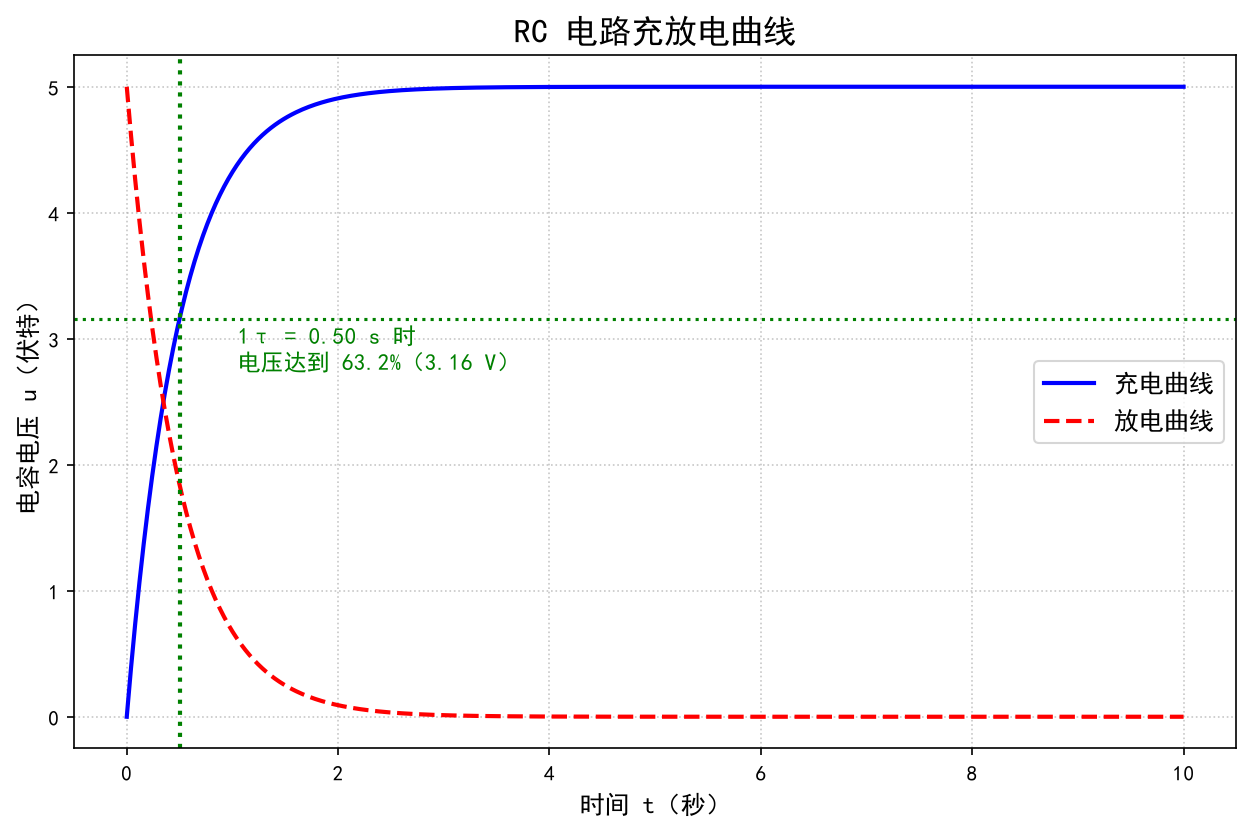
\includegraphics[width=0.8\textwidth]{RC充放电曲线.png}
\caption{RC 电路充放电波形（此处插入示波器截图或 Python 生成的图）}
\label{fig:wave}
\end{figure}

\subsection{误差分析}
实测值与理论值存在约 $1.7\%$ 的偏差，主要原因有：

\begin{enumerate}
    \item 电阻、电容本身存在标称误差（一般 $\pm 5\%$）；
    \item 示波器读数存在人为判读误差；
    \item 电容存在漏电流，并非理想元件。
\end{enumerate}

\section{实验结论}
\begin{enumerate}
    \item RC 电路的充放电过程符合指数规律，与式~\eqref{eq:charge}、\eqref{eq:discharge} 一致；
    \item 实测时间常数 $0.997\ \mathrm{s}$ 与理论值 $1.00\ \mathrm{s}$ 基本吻合；
    \item 验证了时间常数公式 $\tau = RC$ 的正确性。
\end{enumerate}

% ---------- 参考文献（可选）----------
\begin{thebibliography}{9}
\bibitem{book1} 邱关源. 电路[M]. 第5版. 北京: 高等教育出版社, 2006.
\bibitem{book2} 康华光. 电子技术基础（模拟部分）[M]. 北京: 高等教育出版社, 2013.
\end{thebibliography}

\end{document}
